% Chapter Template

% Main chapter title
%\chapter[toc version]{doc version}
\chapter{Testing \& Evaluation}

% Short version of the title for the header
%\chaptermark{version for header}

% Chapter Label
% For referencing this chapter elsewhere, use \ref{ChapterTemplate}
\label{Chapter6TestingEvaluation}

This chapter evaluates the system's performance and practical usability.

The first part of the chapter  evaluates the system's performance across three implementations: Flask, Flask + Celery, 
and FastAPI. The aim is to assess whether transitioning to an asynchronous architecture yields measurable improvements in 
execution time and consistency, particularly for\ac{vm} lifecycle operations such as creation, cloning, and deletion.

Benchmark tasks representative of system usage for recurring tasks are executed under controlled conditions. Results are analyzed 
based on average execution time and variability.

During this process, however, we also encountered infrastructure-level issues unrelated to the choice of framework. In particular, 
I/O bottlenecks on the\ac{pve} node emerged during intensive batch operations, prompting a closer investigation.

The second part provides a walkthrough of the main functional use cases supported by the system from an end-user perspective. 
Given the early-stage, prototypical nature of the user interface and the absence of structured usability testing, the focus here 
is on illustrating how the system is used to perform key operations. Mapping to the functional requirements described in 
Chapter~\ref{Chapter4SystemArchitectureDesign}, thereby serving as a practical validation of the implemented features.

It is important to clarify that the evaluation presented in this work primarily focuses on infrastructure-level operations, 
such as cloning, starting, and deleting\ac{vm}s on\ac{pve}. While the system also automates and interacts with \ac{gns3} 
instances, particularly for tasks such as topology validation athese aspects were not the primary subject of performance 
evaluation. The rationale is that\ac{gns3}-level interactions occur after infrastructure provisioning and are more tightly 
coupled to exercise-specific logic, rather than the orchestration layer itself. As such, the current analysis emphasizes the 
efficiency and scalability of core\ac{vm} management rather than the behavior of individual emulated network devices.

Finally, Flask's synchronous request model under\ac{wsgi} can become a bottleneck in disk-intensive scenarios, particularly when 
backed by a single\ac{ssd}. While modern\ac{ssd}s support parallel I/O at the hardware level, Flask processes requests sequentially 
per worker, preventing full utilization of this parallelism. In contrast, asynchronous frameworks allow concurrent I/O within a single 
thread, offering more efficient resource usage in I/O-bound workloads.


\section{Performance Evaluation}

    To evaluate the impact of migrating from Flask (+ Celery) to FastAPI, we conducted a series of measurements 
    focused on two main performance metrics:

    \begin{itemize}
        \item \textbf{Time to complete a given task}.
        \item \textbf{Consistency of that time}.
    \end{itemize}

    To collect data for analysis we divised three different tasks. Although our evaluation focused on isolated 
    task execution, it is important to note that the use of FastAPI and the\ac{asgi} server model introduces 
    architectural advantages beyond just concurrent task handling. In particular, it can improve response 
    times when multiple students simultaneously interact with the system (e.g., during an exam). While this 
    scenario was not explicitly tested, given the complexity of simulating realistic concurrent user behavior, 
    it remains a key motivation for adopting an asynchronous framework.

    \subsection{Available Hardware}

        The current test environment hosts all internal system components on a single physical server with the 
        following specifications.

        \begin{table}[h]
            \centering
            \caption{System Hardware Specifications}
            \begin{tabular}{|l|l|}
                \hline
                \textbf{Component} & \textbf{Specification} \\ \hline
                Processor & Intel Core i7-9700K \\ \hline
                Memory & 32GB DDR4 @ 2666MHz \\ \hline
                Storage & 1TB Samsung 970 EVO Plus NVMe\ac{ssd} \\ \hline
                Graphics & NVIDIA GTX 1650 \\ \hline
            \end{tabular}
        \end{table}

        This machine's specifications, while capable enough for development purposes, create inherent memory constraints. With 32GB of available RAM, 
        practical\ac{vm} allocation becomes the primary bottleneck. For instance, when deploying\ac{gns3} instances each configured with 4GB of memory, 
        the system can maintain only seven active\ac{vm}s simultaneously. This limitation accounts for\ac{pve}'s own memory overhead 
        before inducing SWAP file usage, which would degrade performance.

    

    \begin{enumerate}
        \item \textbf{1st task: Template\ac{vm} creation:} Create a linked clone from a pre-configured template. Once 
        the cloning process is complete, the\ac{vm} is powered on and polled periodically until a valid IP address is 
        obtained. A \texttt{gns3project} file is then imported into its\ac{gns3} instance. After the import completes, 
        the\ac{vm} is powered off and converted into a reusable template\ac{vm}.

        \item \textbf{2nd task: Batch\ac{vm} cloning:} Generate a specified number of linked clones from an existing template\ac{vm}, 
        each intended for assignment to a different user.

        \item \textbf{3rd task: Batch\ac{vm} deletion:} Remove all cloned\ac{vm}s associated with an exercise, as well as 
        the corresponding template\ac{vm}.

    \end{enumerate}

    Each batch test was conducted using different quantities of\ac{vm} clones: 1, 10, 20, 100, and 200. All data is available at: 
    \url{https://docs.google.com/spreadsheets/d/e/2PACX-1vR08HiAzAyZFhjHRZl-iAnkf748y9e9-5lj-sVstbKX41DxEHpz27TJ7tb7pQBozbF6Xtq-ktSnIE5_/pubhtml}
    

    All three implementations were deployed in the same network environment, hardware and with as minimal differences in code 
    as possible to ensure a fair comparison. The web application in each case was hosted within the same container running 
    on the same host machine. The container was allocated 8 virtual\ac{cpu} cores and 1GB of RAM.

    Time measurements were recorded from the start of a task's execution, defined as the moment the first relevant\ac{api} 
    request was issued, until the moment of successful completion, when the final\ac{api} response was received.

    For the first task, each implementation was run a total of fifteen times.

    For the remaining two scenarios, tests were repeated three times for each implementation and batch size combination. The reported values represent 
    the average across these repetitions. While three runs may not provide the statistical robustness of a larger sample size, they are sufficient to 
    identify consistent trends and relative performance differences. Due to time constraints, more extensive testing was not feasible at this stage.

    For the FastAPI implementation, a concurrency limit of 5 was imposed for interactions with the\ac{pve}\ac{api} for reasons 
    that will be discussed in Section~\ref{sec:io_problems}. 
    Other categories of tasks, such as user requests,\ac{gns3} project handling, and Nornir automation, were allowed to 
    proceed without any concurrency restrictions.

        \subsubsection{Task 1: Template VM Creation}

            This task is sequential in nature, as it interacts with only a single\ac{vm}, and none of the steps can be performed in 
            parallel, as each step depends on the previous one. As such, no significant performance uplift is expected for this particular 
            task.

            \begin{figure}[ht]
                \centering
                \begin{tikzpicture}
                    \begin{axis}[
                        title={Comparison of Average Execution Time (in seconds) (n=15)},
                        ybar,
                        bar width=12pt,
                        enlargelimits=0.12,
                        ylabel={Time (s)},
                        xlabel={},
                        xtick=data,
                        xticklabels={},
                        ymin=0,
                        legend style={at={(0.5,-0.15)}, anchor=north, legend columns=-1},
                        ylabel near ticks,
                        xlabel near ticks,
                        nodes near coords,
                        every node near coord/.append style={font=\scriptsize},
                        width=0.6\textwidth,
                        height=7cm,
                    ]

                    % Flask
                    \addplot+[style={blue, fill=blue!30}, bar shift=-18pt] 
                        coordinates {(Impl, 36.942013)};

                    % Flask + Celery
                    \addplot+[style={red, fill=red!30}, bar shift=0pt] 
                        coordinates {(Impl, 34.927078)};

                    % FastAPI
                    \addplot+[style={green!70!black, fill=green!40}, bar shift=18pt] 
                        coordinates {(Impl, 32.197323)};

                    \legend{Flask, Flask + Celery, FastAPI}
                    \end{axis}
                \end{tikzpicture}
                \caption{Average execution time for Template VM creation across implementations.}
                \label{fig:task1_plot}
            \end{figure}

            As can be confirmed in Figure~\ref{fig:task1_plot} the average execution times are very similar across all three implementations, 
            with the FastAPI approach showing a slight performance advantage.

            However, averages alone do not tell the full story. Figure~\ref{fig:task1_boxplot} illustrates the execution time variability. 
            \textit{Note: the y-axis does not start at 0.}

            \begin{figure}[ht]
                \centering
                \begin{tikzpicture}
                    \begin{axis}[
                            title={Execution Time Variability for Template VM Creation (n=15)},
                            ylabel={Time (s)},
                            boxplot/draw direction=y, % Vertical boxplot
                            xtick={1,2,3},
                            xticklabels={Flask, Flask + Celery, FastAPI},
                            width=1\textwidth,
                            height=6cm,
                        ]

                        % First dataset: Flask
                        \addplot+[boxplot] table[row sep=\\,y index=0] {
                        34.364366\\ 34.170579\\ 34.233161\\ 34.373219\\ 34.172813\\
                        34.187679\\ 45.605793\\ 45.336995\\ 34.179929\\ 45.598744\\
                        34.215090\\ 34.188849\\ 34.329254\\ 35.997439\\ 39.176289\\
                        };

                        % Second dataset: Flask + Celery
                        \addplot+[boxplot] table[row sep=\\,y index=0] {
                        34.415269\\ 34.181023\\ 34.204050\\ 34.469319\\ 34.203889\\
                        34.207585\\ 34.426887\\ 34.223055\\ 34.390095\\ 34.433466\\
                        34.194064\\ 34.224277\\ 34.412016\\ 38.699065\\ 39.222109\\ 
                        };

                        % Third dataset: FastAPI
                        \addplot+[boxplot] table[row sep=\\,y index=0] {
                        32.277591\\ 32.137275\\ 32.247606\\ 32.213745\\ 32.216619\\ 
                        32.155424\\ 32.249668\\ 32.165283\\ 32.138648\\ 32.169642\\
                        32.208805\\ 32.235647\\ 32.203489\\ 32.156690\\ 32.183706\\ 
                        };

                    \end{axis}
                \end{tikzpicture}
                \caption{Boxplot comparison of execution time variability for Template VM creation.}
                \label{fig:task1_boxplot}
            \end{figure}

            From the boxplot, it is evident that the Flask implementation exhibits the highest 
            variability in execution times, indicating inconsistency. The Flask + Celery variant improves consistency but still 
            contains several statistical outliers. In contrast, the FastAPI implementation demonstrates significantly tighter 
            grouping and no outliers in our tests.

            This coupled with the slighty better execution time make the FastAPI implementation the more performant of 
            the three.

        \subsubsection{Task 2: VM Cloning}            
            Unlike the previous task, the cloning of multiple\ac{vm}s can be executed concurrently, as each cloning operation 
            consists of only two main steps and is entirely independent from the others.

            For each\ac{vm}, a random ID is first selected, followed by an\ac{api} call to\ac{pve} to verify that the ID is not already 
            in use. Given the large available range (100 to 999999999), and our comparatively small usage of them, collisions are rare, 
            and the check typically succeeds immediately. In the event of a colision at any point, another random ID is generated and 
            retried until success.

            Once a free ID is confirmed, a second\ac{api} call to\ac{pve} is made to clone the\ac{vm} using that ID. Because these two 
            calls are independent for each\ac{vm}, the cloning process can be parallelized with minimal coordination or contention overhead.

            \begin{figure}[ht]
                \centering
                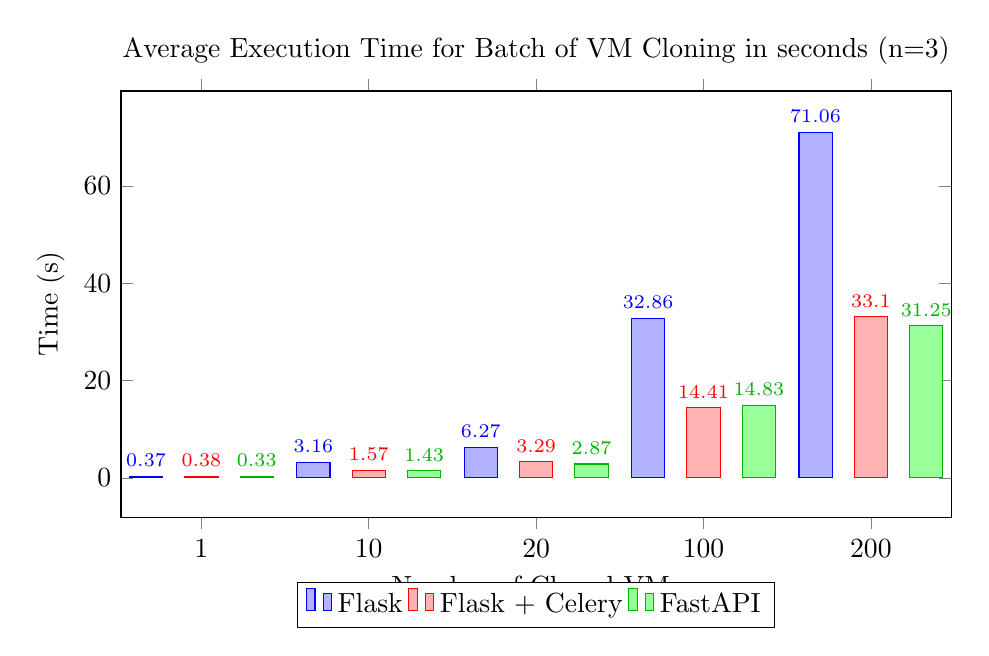
\begin{tikzpicture}
                    \begin{axis}[
                        title={Average Execution Time for Batch of VM Cloning in seconds (n=3)},
                        ybar,
                        bar width=12pt,
                        enlargelimits=0.12,
                        ylabel={Time (s)},
                        xlabel={Number of Cloned VMs},
                        symbolic x coords={1, 10, 20, 100, 200},
                        xtick=data,
                        legend style={at={(0.5,-0.15)}, anchor=north, legend columns=-1},
                        ylabel near ticks,
                        xlabel near ticks,
                        nodes near coords,
                        every node near coord/.append style={font=\scriptsize},
                        width=1\textwidth,
                        height=7cm,
                    ]

                    % Example dummy data: replace these values with your actual measurements

                    % Flask
                    \addplot+[style={blue, fill=blue!30}, bar shift=-20pt] plot coordinates {
                        (1, 0.368690)
                        (10, 3.163624)
                        (20, 6.265722)
                        (100, 32.864042)
                        (200, 71.062075)
                    };

                    % Flask + Celery
                    \addplot+[style={red, fill=red!30}, bar shift=0pt] plot coordinates {
                        (1, 0.377741)
                        (10, 1.565772)
                        (20, 3.287195)
                        (100, 14.412073)
                        (200, 33.095232)
                    };

                    % FastAPI
                    \addplot+[style={green!70!black, fill=green!40}, bar shift=20pt] plot coordinates {
                        (1, 0.330939)
                        (10, 1.434924)
                        (20, 2.872174)
                        (100, 14.832606)
                        (200, 31.253715)
                    };

                    \legend{Flask, Flask + Celery, FastAPI}
                    \end{axis}
                \end{tikzpicture}
                \caption{Average execution time to clone increasing number of\ac{vm}s across different implementations.}
                \label{fig:task2_plot}
            \end{figure}

            From Figure~\ref{fig:task2_plot}, we observe that the task completion time increases linearly with the number of 
            \ac{vm}s. The purely sequential Flask implementation consistently underperforms compared to the other two approaches, 
            except in the smallest batch size test, where no concurrency can be achieved.

            To compare the consistency of different implementations (Flask, Flask+Celery, FastAPI) across batch sizes, we first 
            normalize each run's execution time within its batch. For each combination of implementation and batch size, compute 
            the batch mean of the run times. Then calculate each run's percentage deviation from that mean using the standard 
            percent-change formula:

            \[
            \text{Deviation}_i = \frac{\text{time}_i - \text{batch\_mean}}{\text{batch\_mean}} \times 100\%.
            \]

            This normalization step effectively centers each batch's data at zero and removes scale differences. For example, 
            if a run is 10\,ms above a 100\,ms mean, its deviation is 
            \[
            \frac{10}{100} \times 100 = 10\%.
            \]
            This ensures that larger batch sizes, which naturally require more time, do not dominate the analysis. Instead, we 
            focus on the relative fluctuations around each batch's mean.

            \begin{figure}[ht]
                \centering
                \begin{tikzpicture}
                    \begin{axis}[
                            title={Execution Time Deviation for Batch VM Cloning (n=3)},
                            ylabel={Deviation (\%)},
                            boxplot/draw direction=y, % Vertical boxplot
                            xtick={1,2,3},
                            xticklabels={Flask,Flask + Celery,FastAPI},
                            width=1\textwidth,
                            height=6cm,
                        ]

                        % First dataset: Flask
                        \addplot+[boxplot] table[row sep=\\,y index=0] {
                         3.221134\\  0.112139\\ 1.133900\\
                        1.021761\\ 0.800631\\ 1.463433\\ 0.662802\\ 0.175874\\
                        0.020318\\ 0.196192\\ 0.151488\\ 0.440729\\ 0.592217\\
                        };

                        % Second dataset: Flask + Celery
                        \addplot+[boxplot] table[row sep=\\,y index=0] {
                        1.454436\\ 0.773281\\ 2.227717\\ 0.933618\\ 4.111049\\
                        3.177431\\ 5.191073\\ 1.166758\\
                        0.786188\\ 1.952946\\ 5.706726\\ 1.309611\\ 4.397116\\
                        };

                        % Third dataset: FastAPI
                        \addplot+[boxplot] table[row sep=\\,y index=0] {
                        0.493747\\ 3.698869\\ 3.205122\\ 1.216185\\ 0.476169\\
                        0.740016\\ 1.803419\\ 2.513543\\ 4.316962\\ 0.408508\\
                        0.784985\\ 0.376477\\ 0.903063\\ 2.445461\\ 1.542398\\
                        };

                    \end{axis}
                \end{tikzpicture}
                \caption{Boxplot comparison of execution time variability for VM cloning.}
                \label{fig:task2_boxplot}
            \end{figure}

            Once again, in Figure~\ref{fig:task2_boxplot}, we observe the same trend: the FastAPI implementation is slightly 
            faster and more consistent when compared to the Flask + Celery approach, altought the Flask sequential implementation 
            actually wins in this metric of deviation, being more consistent than the other two in run-to-run variation, at the cost of 
            being two times slower than the FastAPI implementation, making the FastAPI effort the overall better performer.


        \subsubsection{Task 3: VM Deletion}

            This task is much more short lived than the previous ones, consisting of a single\ac{api} call to\ac{pve} per\ac{vm} to 
            perform the deletion.

            Since the deletion operation does not require any preliminary validation or resource allocation, each\ac{vm} can be 
            removed independently without the need for coordination. This simplicity allows for rapid execution and straightforward 
            parallelization of the deletion process, with minimal overhead per\ac{vm}.
                        

            \begin{figure}[ht]
                \centering
                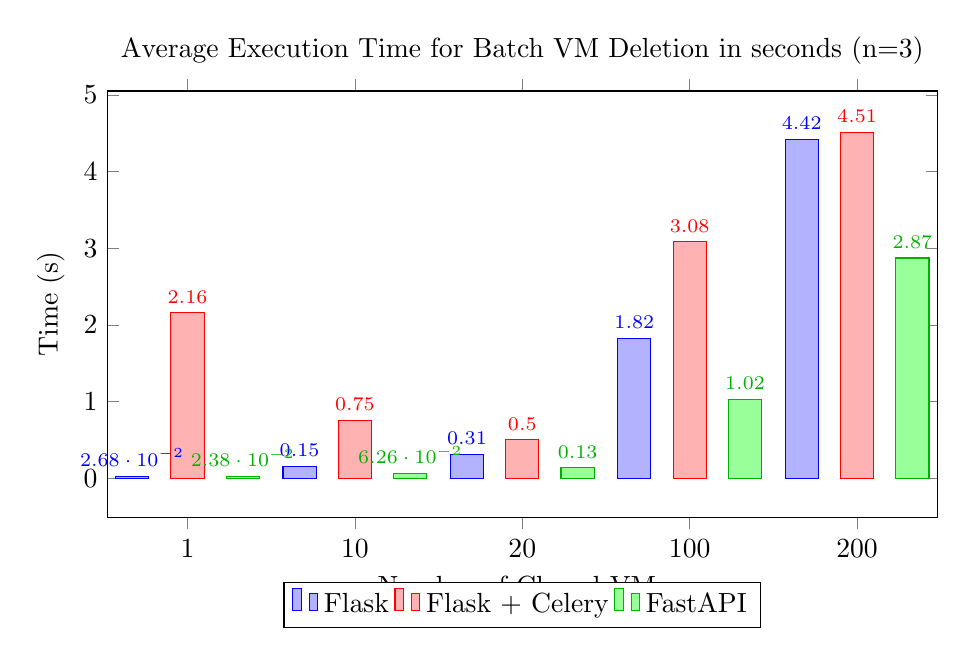
\begin{tikzpicture}
                    \begin{axis}[
                        title={Average Execution Time for Batch VM Deletion in seconds (n=3)},
                        ybar,
                        bar width=12pt,
                        enlargelimits=0.12,
                        ylabel={Time (s)},
                        xlabel={Number of Cloned VMs},
                        symbolic x coords={1, 10, 20, 100, 200},
                        xtick=data,
                        legend style={at={(0.5,-0.15)}, anchor=north, legend columns=-1},
                        ylabel near ticks,
                        xlabel near ticks,
                        nodes near coords,
                        every node near coord/.append style={font=\scriptsize},
                        width=1\textwidth,
                        height=7cm,
                    ]

                    % Flask
                    \addplot+[style={blue, fill=blue!30}, bar shift=-20pt] plot coordinates {
                        (1, 0.026849)
                        (10, 0.153751)
                        (20, 0.312510)
                        (100, 1.820313)
                        (200, 4.418675)
                    };

                    % Flask + Celery
                    \addplot+[style={red, fill=red!30}, bar shift=0pt] plot coordinates {
                        (1, 2.155812)
                        (10, 0.753148)
                        (20, 0.500132)
                        (100, 3.084107)
                        (200, 4.513475)
                    };

                    % FastAPI
                    \addplot+[style={green!70!black, fill=green!40}, bar shift=20pt] plot coordinates {
                        (1, 0.023758)
                        (10, 0.062618)
                        (20, 0.134784)
                        (100, 1.022950)
                        (200, 2.872160)
                    };

                    \legend{Flask, Flask + Celery, FastAPI}
                    \end{axis}
                \end{tikzpicture}
                \caption{Average execution time to delete increasing number of\ac{vm}s across different implementations.}
                \label{fig:task3_plot}
            \end{figure}

            In Figure~\ref{fig:task3_plot} we can see a textbook example of the overhead that Celery and the message broker 
            bring with them, and why it is not a good idea to use them for especially short-lived, non-\ac{cpu} intensive tasks. 
            The additional overhead introduced significantly impacts the overall execution time. 

            In this case, those two factors, the asynchronous orchestration and broker communication, have a higher influence on 
            execution time than the\ac{vm} batch size itself.

            In the particular case of sample size 1, we can see that it took even more time than bigger batch sizes. While this 
            may in part be fault of our relatively small data pool, we choose to keep it as it highlights very well the performance 
            overhead that celery brings with it, and why it can be considered detrimental in the case of short-lived tasks

            When comparing batch size 100 to 200, FastAPI exhibited a 2.8x slowdown despite only a 2x increase in workload. This disproportional 
            latency is not due to FastAPI itself, but rather to hitting performance limits in\ac{pve}. As infrastructure resources became saturated, 
            clone operations began failing and triggered exponential backoff retries, leading to higher cumulative delays.

            The other implementations scale in a much more expected manner, with the FastAPI version being 1.84x faster on average 
            than Flask.

            \begin{figure}[ht]
                \centering
                \begin{tikzpicture}
                    \begin{axis}[
                            title={Execution Time Deviation for Batch VM Deletion (n=3)},
                            ylabel={Deviation (\%)},
                            boxplot/draw direction=y, % Vertical boxplot
                            xtick={1,2,3},
                            xticklabels={Flask,Flask + Celery,FastAPI},
                            width=1\textwidth,
                            height=6cm,
                        ]

                        % First dataset: Flask
                        \addplot+[boxplot] table[row sep=\\,y index=0] {
                        1.466243\\ 0.254513\\ 1.211730\\ 1.705134\\ 0.029702\\ 
                        1.734836\\ 0.053972\\ 2.575067\\ 2.521095\\ 0.877047\\
                        0.594293\\ 1.471340\\ 0.669756\\ 0.299788\\ 0.369968\\
                        };

                        % Second dataset: Flask + Celery
                        \addplot+[boxplot] table[row sep=\\,y index=0] {
                        0.054210\\ 46.458512\\ 46.404302\\ 178.150500\\ 89.246465\\
                        88.904035\\ 69.954352\\ 135.324717\\ 65.370365\\ 64.345415\\
                        0.149854\\ 64.495269\\ 34.231252\\ 8.277547\\ 25.953705\\
                        };

                        % Third dataset: FastAPI
                        \addplot+[boxplot] table[row sep=\\,y index=0] {
                        1.491407\\ 2.526833\\ 4.018239\\ 0.849068\\ 6.666383\\
                        5.817315\\ 4.301698\\ 1.202665\\ 3.099033\\ 0.149600\\
                        0.913567\\ 1.063167\\ 0.735265\\ 0.763815\\ 0.028550\\
                        };

                    \end{axis}
                \end{tikzpicture}
                \caption{Boxplot comparison of execution time variability for VM deletion.}
                \label{fig:task3_boxplot}
            \end{figure}

            As shown in Figure~\ref{fig:task3_boxplot}, the Flask + Celery implementation exhibits significantly higher variability 
            during this task when compared to the other two approaches. The presence of numerous outliers and a wide interquartile range 
            highlight the inconsistency introduced by Celery and the message broker's overhead.

            \begin{figure}[ht]
                \centering
                \begin{tikzpicture}
                    \begin{axis}[
                            title={Execution Time Deviation for Batch VM Deletion (n=3)},
                            ylabel={Deviation (\%)},
                            boxplot/draw direction=y, % Vertical boxplot
                            xtick={1,2},
                            xticklabels={Flask,FastAPI},
                            width=1\textwidth,
                            height=6cm,
                        ]

                        % First dataset: Flask
                        \addplot+[boxplot] table[row sep=\\,y index=0] {
                        1.466243\\ 0.254513\\ 1.211730\\ 1.705134\\ 0.029702\\ 
                        1.734836\\ 0.053972\\ 2.575067\\ 2.521095\\ 0.877047\\
                        0.594293\\ 1.471340\\ 0.669756\\ 0.299788\\ 0.369968\\
                        };

                        % Third dataset: FastAPI
                        \addplot+[boxplot] table[row sep=\\,y index=0] {
                        1.491407\\ 2.526833\\ 4.018239\\ 0.849068\\ 6.666383\\
                        5.817315\\ 4.301698\\ 1.202665\\ 3.099033\\ 0.149600\\
                        0.913567\\ 1.063167\\ 0.735265\\ 0.763815\\ 0.028550\\
                        };

                    \end{axis}
                \end{tikzpicture}
                \caption{Boxplot comparison of execution time variability of Flask and FastAPI for VM deletion.}
                \label{fig:task3_boxplot2}
            \end{figure}

            Figure~\ref{fig:task3_boxplot2} isolates the Flask and FastAPI implementations for a clearer comparison. We observe that while 
            the Flask approach is slightly more consistent, as indicated by its tighter distribution.
        
    \subsection{I/O Problems during Batch VM Operations}
    \label{sec:io_problems}

        \begin{figure}[h]
        \centering
        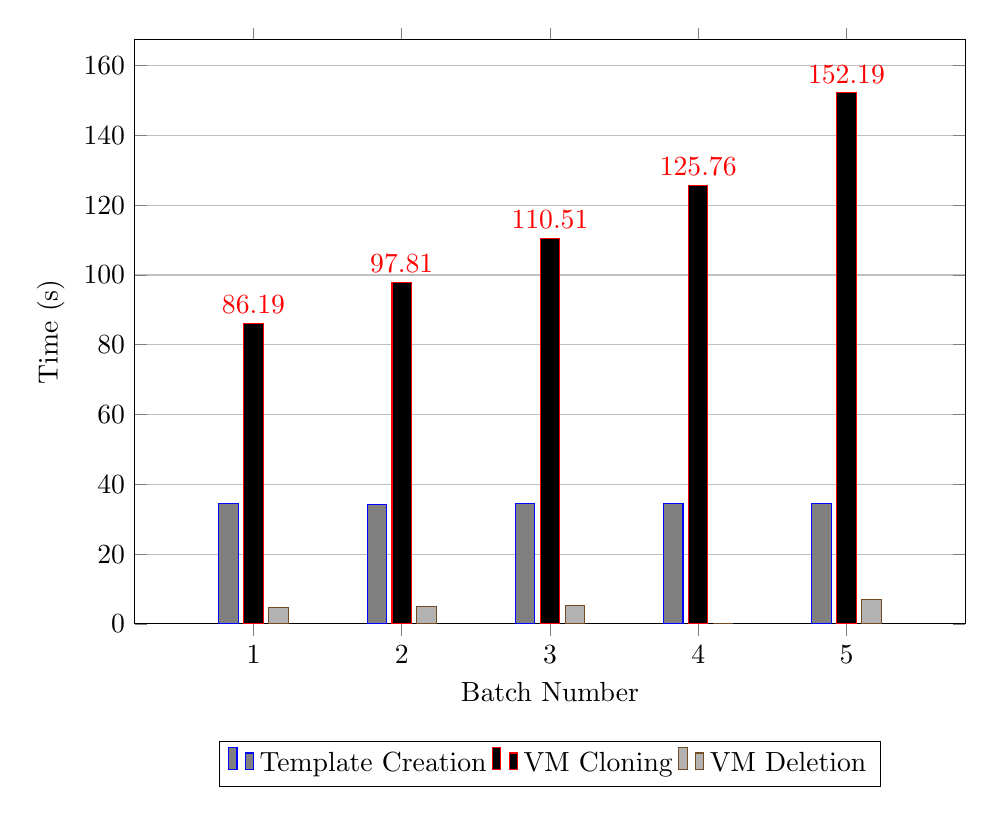
\begin{tikzpicture}
            \begin{axis}[
            ybar,
            bar width=7pt,
            width=\textwidth,
            height=9cm,
            ylabel={Time (s)},
            xlabel={Batch Number},
            symbolic x coords={1,2,3,4,5},
            xtick=data,
            ymin=0,
            enlarge x limits=0.2,
            legend style={at={(0.5,-0.2)}, anchor=north,legend columns=3},
            ymajorgrids=true,
            bar shift auto
            ]

                % Template creation (no labels)
                \addplot+[ybar, fill=gray] coordinates {
                (1,34.379) (2,34.312) (3,34.422) (4,34.609) (5,34.571)
                };
                \addlegendentry{Template Creation}

                % VM cloning (with labels)
                \addplot+[
                ybar,
                fill=black,
                nodes near coords,
                ] coordinates {
                (1,86.187) (2,97.805) (3,110.508) (4,125.758) (5,152.186)
                };
                \addlegendentry{VM Cloning}

                % VM deleting (no labels)
                \addplot+[ybar, fill=gray!60] coordinates {
                (1,4.612) (2,4.942) (3,5.377) (4,0.0) (5,7.090)
                };
                \addlegendentry{VM Deletion}

                \end{axis}
            \end{tikzpicture}
            \caption{Grouped bar chart showing VM operation times. Cloning time is labeled to highlight the rising trend. Results
            from Flask running purely sequential code}
            \label{fig:io_grouped_bar_plot}
        \end{figure}

        During initial stress tests of batch cloning and deletion of\ac{vm}s, 200 at a time, on our single node\ac{pve} cluster, 
        we observed rising task times in subsequent runs, specifically for the mass cloning of new\ac{vm}s, as can be seen in 
        Figure~\ref{fig:io_grouped_bar_plot}.

        It was also noted that there was an error thrown by\ac{pve} during the 4th batch of tasks, specifically during the 
        deleting task, causing it to fail.

        After some investigation it was found that there were intermittent failures to remove\ac{vm} disks. These failures 
        were \emph{not} detectable via the\ac{pve}\ac{http}\ac{api} responses and only appeared in the\ac{pve} server 
        logs. As orphaned disks accumulated, overall performance degraded significantly.
        \medskip

        \noindent\textbf{Observed Task History Outputs:}

\paragraph{1st type of output:} disk removed successfully

        \begin{verbatim}
trying to acquire lock...
OK
Logical volume "vm-348786940-disk-0" successfully removed.
TASK OK
        \end{verbatim}

\paragraph{2nd type of output:} intermittent lock-timeout failures followed by disk removed successfully

        \begin{verbatim}
trying to acquire lock...
Could not remove disk 'local-lvm:vm-120993831-disk-0', check manually:
can't lock file '/var/lock/pve-manager/pve-storage-local-lvm' - got timeout
trying to acquire lock...
OK
Logical volume "vm-120993831-disk-0" successfully removed.
TASK OK
        \end{verbatim}
        
\paragraph{ 3rd type of output:} failure to remove disk

        \begin{verbatim}
trying to acquire lock...
Could not remove disk 'local-lvm:vm-363495383-disk-0', check manually:
can't lock file '/var/lock/pve-manager/pve-storage-local-lvm' - got timeout
trying to acquire lock...
can't lock file '/var/lock/pve-manager/pve-storage-local-lvm' - got timeout
TASK OK
        \end{verbatim}

\paragraph{4th and final type of output:} storage config update errors and failure to remove disk

        \begin{verbatim}
trying to acquire lock...
Could not remove disk 'local-lvm:vm-5469324-disk-0', check manually:
can't lock file '/var/lock/pve-manager/pve-storage-local-lvm' - got timeout
trying to acquire lock...
can't lock file '/var/lock/pve-manager/pve-storage-local-lvm' - got timeout
trying to acquire cfs lock 'file-user_cfg' ...
TASK OK
        \end{verbatim}
                
        This suggests\ac{pve}'s locking mechanism can't keep pace with big amounts of deletion requests in quick succession.. 
        The lock is used to ensure that two tasks dont modify the\ac{lvm}'s metadata simulatenously. Since there should be 
        some underlying I/O tasks that are piling up, the system can't keep pace and eventually starts resorting to a retry mechanism 
        to keep up, but even this is insuficient and starts failing more and more towards the end as it becomes fully congested. 
        At the end, the system starts becoming overwhelmed and also begins having trouble updating its internal storage 
        config file.  

        This, combined with other factors were the main reason that led us to implement a hard limit on the amount of concurrent 
        requests that can be made from the web application to\ac{pve}\ac{api}. Still, while this significantly reduces the chances 
        of this problem reocurring, it does not fully remedy the problem and additional future work should look into solving this 
        matter completely.



        \begin{figure}[h]
        \centering
        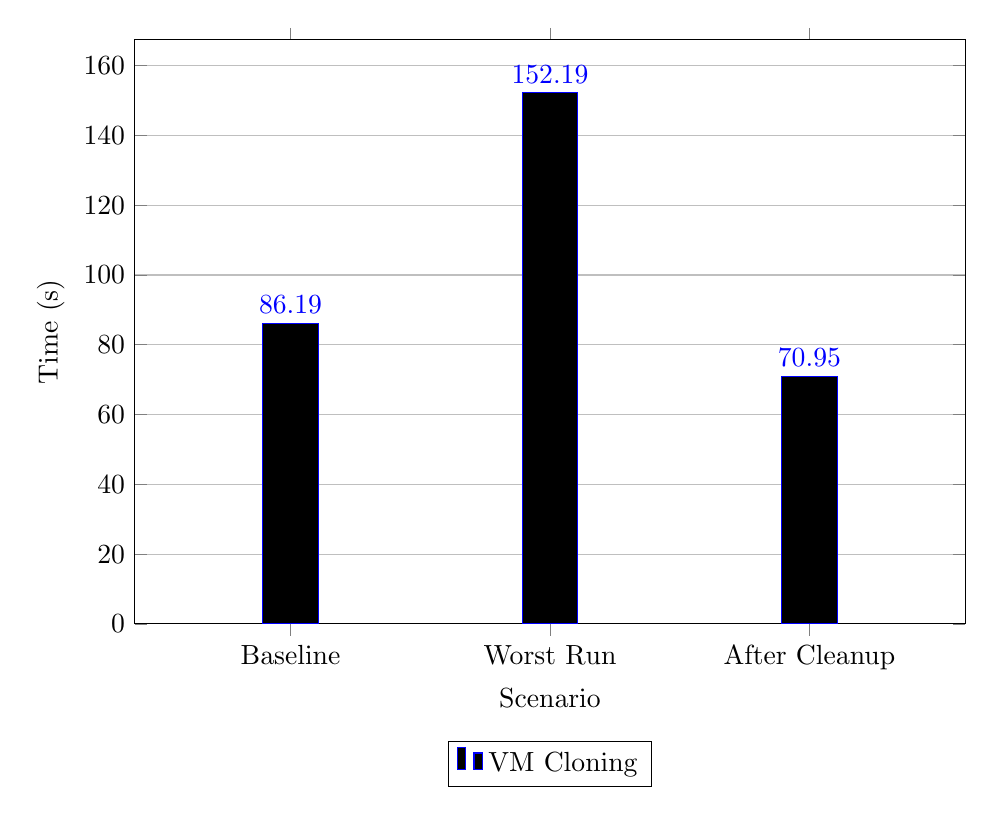
\begin{tikzpicture}
            \begin{axis}[
                ybar,
                bar width=20pt,
                width=\textwidth,
                height=9cm,
                ylabel={Time (s)},
                xlabel={Scenario},
                symbolic x coords={Baseline,Worst Run,After Cleanup},
                xtick=data,
                ymin=0,
                enlarge x limits=0.3,
                legend style={at={(0.5,-0.2)}, anchor=north, legend columns=1},
                ymajorgrids=true,
                nodes near coords
            ]

            % VM cloning bars without labels
            \addplot+[
                ybar,
                fill=black
            ] coordinates {
                (Baseline,86.187)
                (Worst Run,152.186)
                (After Cleanup,70.954)
            };
              
            \addlegendentry{VM Cloning}

            \end{axis}
        \end{tikzpicture}
        \caption{Bar chart showing VM cloning times after cleanup, at baseline, and in the worst case scenario.}
        \label{fig:vm_grouped_cloning_focus}
        \end{figure}

        After writing a small script to perform a cleanup of the orphaned disks we can see in 
        Figure~\ref{fig:vm_grouped_cloning_focus} that performance was improved from even our 1st recorded baseline test.

\section{System Usage}
    Due to the very early and prototipical\ac{ui} developed for the web application as well as lack of time to gather users in 
    order to perform usability tests, this section will contain a guide on how to perform various use cases.

    \subsection{Create a new exercise and enroll students}
        To start, the user must provide privileged credentials using the login form shown in Figure~\ref{fig:web_app_login}. 
        Without authorized credentials, the web application will not authorize the creation of new exercises.

        \begin{figure}
            \centering
            \includegraphics[width=5cm]{6TestingEvaluation/web_app_login.png}
            \caption{A screenshot of the login page}
            \label{fig:web_app_login}
        \end{figure}

        Next, the user should navigate to the ``Exercises" page via the navigation bar, and then select ``Create Exercise". This 
        will display the form shown in Figure~\ref{fig:web_app_create_exercise}.

        \begin{figure}
            \centering
            \includegraphics[width=10cm]{6TestingEvaluation/web_app_create_exercise.png}
            \caption{ A screenshot of the create exercise page}
            \label{fig:web_app_create_exercise}
        \end{figure}

        The form includes the following key fields:
        
        \begin{itemize}
             \item \textbf{Template VM Proxmox ID}:  This refers to the Proxmox ID of the template\ac{vm} to be cloned. 
             The template must meet the previously defined requirements: it should have\ac{gns3} installed and configured 
             to start automatically after boot, and it should contain the necessary network devices.
             \item \textbf{GNS3 Project File}: This field accepts a file with the \texttt{gns3project} extension, which can be exported 
             directly from\ac{gns3}.
             \item \textbf{Exercise validation}: This field allows the user to define one or more validation checks to be executed 
             on the specified devices. Currently, only \texttt{ping} and \texttt{traceroute} commands are supported. These validations will be executed 
             when a student requests automatic assessment.
             \item \textbf{Exercise pre-configuration}: This field enables the execution of custom commands on any supported device type 
             for initial configuration. These commands will be executed only on the template\ac{vm} before it is converted into a reusable 
             template.
        \end{itemize}

        After completing this process, clearing the functional use case described in Subsection~\ref{sec:new_exercise},the user should navigate to 
        the newly created exercises' page, as shown in Figure~\ref{fig:web_app_exercise}, and click on "Manage Exercise".

        \begin{figure}
            \centering
                \includegraphics[width=5cm]{6TestingEvaluation/web_app_exercise.png}
            \caption{ A screenshot of the exercise page}
            \label{fig:web_app_exercise}
        \end{figure}

        In the management interface (Figure~\ref{fig:web_app_manage_exercise}), the user can enroll or remove students from the exercise. Enrolling a 
        student automatically creates and assigns a dedicated\ac{vm}, completing the use case in Subsection~\ref{sec:enlist_users}, while removing them 
        destroys the corresponding\ac{vm}. It is important to note that exercises are only visible to students who are enrolled in them.

        \begin{figure}
            \centering
            \includegraphics[width=8cm]{6TestingEvaluation/web_app_manage_exercise.png}
            \caption{ A screenshot of the exercise management page}
            \label{fig:web_app_manage_exercise}
        \end{figure}

    \subsection{Complete an assignment and request an assessment}

        To begin, the user must log in using the form shown in Figure~\ref{fig:web_app_login}, ensuring the account is enrolled in at least one exercise. 
        After logging in, the user should navigate to the exercises page (Figure~\ref{fig:web_app_exercise}) and click on "Start Work Environment", described in
        Subsection~\ref{sec:starts_vm}.

        Once the environment has been initialized, the user can click on "Connect to Work Environment", which will redirect them to the gns3-web instance 
        hosted on their dedicated\ac{vm} for the selected exercise. Within the\ac{gns3} interface, the user should configure the available devices according 
        to the requirements specified in the exercise description.

        When ready, the user can click "Request Exercise Evaluation" to trigger the automated validation process, which checks whether the exercise has 
        been correctly configured.

        After the assessment is complete, the results are displayed on the page shown in Figure~\ref{fig:web_app_assessment_exercise}, as described in 
        Subsection~\ref{sec:submit_solution}.

        \begin{figure}
            \centering
            \includegraphics[width=10cm]{6TestingEvaluation/web_app_assessment_exercise.png}
            \caption{ A screenshot of the exercise management page}
            \label{fig:web_app_assessment_exercise}
        \end{figure}


% Write text in here
% Use \subsection and \subsubsection to organize text
